\documentclass[prb,preprint]{revtex4-1} 

\usepackage{amsmath}  
\usepackage{amsfonts} 
\usepackage{graphicx} 
\usepackage{color}
\usepackage{ulem}

\begin{document}


\title{}


\author{Danika Luntz-Martin}
\email{dluntzma@smith.edu}
\affiliation{Department of Physics, Smith College, Northampton, MA 01063}

\author{William Williams}
\email{wwilliams@smith.edu} 
\affiliation{Department of Physics, Smith College, Northampton, MA 01063}

\date{\today}

\begin{abstract}


\end{abstract}


\maketitle 


\section{Introduction} 


\section{Theory}

Krypton is one of the noble gases, its outer electron shell is completely filled, as such the energy gap between the ground energy state and the first excited state is large (Add number here). Therefore to laser cool from the ground state would require (123nm?) light which is not currently possible experimentally. To be able to trap krypton atoms they need to be in an excited state and that state needs to be metastable so that the atoms cannot decay while we are cooling and trading them. 

To get the kryptons to the metastable state we used a 215nm light to drive a two-photon transition from the ground $4P^6$ $^1S_0$ state, to the $5P_{[3/2]_2}$ state. Throughout our calculations we call the ground $4P^6$ $^1S_0$ state 'state 1' and the $5P_{[3/2]_2}$ state 'state 2.' There are other states at similar energies to the states in question, but they are not important for our experiment because transitions to them are quantum mechanically forbidden. From the $5P_{[3/2]_2}$ state the atom will either decay to the ground state or it will decay to a metastable state, the $SP_{[3/2]_2}$ state. We called this metastable state 'state 3.' The last possibility is that the atom can ionize either from the the $5P_{[3/2]_2}$ state or the metastable $5S_{[3/2]_2}$ state. \textcolor{blue}{I think I should probably add an image of krypton energy levels.}

Atom trap trace analysis counts atoms that have been trapped so it is limited by the number of atoms in the metastable state, i.e. the number of atoms available to be trapped. To determine the efficiency of our set up, we calculated the percentage of krypton atoms that ended up in the metastable $5S_{[3/2]_2}$ state using the rate equations.

\begin{equation}
\label{RateEq1}
\frac{dN_1}{dt} = -\omega_{12}N_1 + \frac{1}{\tau_{21}}N_2
\end{equation}

Equation~\ref{RateEq1} gives the change in the number of atoms ($N_1$) in the ground state. $\omega_{12}$ is the rate of atoms in state 1 (the ground state) which are excited to state 2, the $5P_{[3/2]_2}$ state, via the two-photon transition. $\omega_{12}$ is negative because atoms are leaving state 1. $\frac{1}{\tau_{21}}$ is the rate of decay from state 2 back to state 1. Similarly, there are differential equations for the three other states.

\begin{equation}
\label{RateEq2}
\frac{dN_2}{dt} = \omega_{12}N_1 -  \frac{1}{\tau_{21}}N_2 - \frac{1}{\tau_{23}}N_2 - R_2N_2
\end{equation}

\begin{equation}
\label{RateEq3}
\frac{dN_3}{dt} =  \frac{1}{\tau_{23}}N_2 - R_3N_3
\end{equation}

\begin{equation}
\label{RateEq4}
\frac{dN_4}{dt} = R_2N_2 + R_3N_3
\end{equation}

Where $\tau_{23}$ if the decay rate from state 3, the metastable state, to state 2. $R_2$ and $R_3$ are the ionization rates from states 2 and 3 respectively. $N_4$ is the number of atoms which have been ionized, just as $N_2$ and $N_3$ are the number of atoms in state 2 and state 3.

Solving these linearly dependent equations is possible, but the computational time is much shorter if they are put into matrix form.

\begin{equation}
\label{RateEqMatrix}
\begin{bmatrix}
	\frac{dN_1}{dt} \\
	\frac{dN_2}{dt} \\
	\frac{dN_3}{dt} \\
	\frac{dN_4}{dt} \\
\end{bmatrix}
=
\begin{pmatrix}
	-\omega_{12} & \frac{1}{\tau_{21}}  & 0 &  0   \\
	\omega_{12}  & -\frac{1}{\tau_{21}}- \frac{1}{\tau_{23}}-R_2 & 0 & 0 \\
	0  &  \frac{1}{\tau_{23}}  & - R_3 & 0 \\
	0  &  R_2  & R_3 & 0  \\
\end{pmatrix}
\begin{bmatrix}
	N_1 \\
	N_2 \\
	N_3 \\
	N_4 \\
\end{bmatrix}
\end{equation}

The general solution to the first order differential matrix equation is \textcolor{blue}{do I need to cite this?}

\begin{equation}
\label{RateEqSol}
N(t) = A_1e^{\lambda_1 t} v_1 + A_2e^{\lambda_2 t} v_2 + A_3e^{\lambda_3 t} v_3 + A_4e^{\lambda_4 t} v_4 
\end{equation}

where $\lambda$ is an eigenvalue of the matrix and v is an eigenvector or the matrix.  A is the amplitude determined by the initial conditions. The initial condition is that all of the atoms are in the ground state, state 1. That is

\begin{equation}
\label{InitialCond}
N_1(0) = 1, \	\	\	\	
N_2(0) = 0, \	\	\	\	
N_3(0) = 0, \	\	\	\	
N_4(0) = 0 
\end{equation}

which allows us to obtain particular solutions to the rate equations. We did all calculations and analysis in Mathematica. \textcolor{blue}{Should I make an appendix with the Mathematica notebooks?} Once we had the solutions to the rate equations we needed to define the variables $\omega_{12}$, $\tau_{21}$, $\tau_{23}$, $R_2$ and $R_3$ which make up the eigenvectors and eigenvalues of the matrix.

\subsection{Constant Intensity and Velocity Approximation} 

For our initial calculation we made a couple simplifying approximations. The first approximation we made was to model the beam profile as constant. The second approximation was to use a single averaged velocity rather then the Maxwell velocity distribution. We later expanded our calculations to account for the beam profile and the velocity distribution those calculations can be found in the subsequent sections. 

The decay rates for state 2 ($5P_{[3/2]_2}$) to state 1 (ground state) and state 3 (metastable state) are know quantities.
\begin{equation}
\label{DecayRates} 
\tau_{21} = 1.1x10^7 s, \	\	\	\	 \tau_{23} = 3.1x10^7s
\end{equation} 
\textcolor{blue}{I think I should cite these, but I am not sure where they came from. Does NIST have these?}

The ionization rates are given by 
\begin{equation}
\label{IonizationRates}
R = \sigma_{pi} \frac{I}{\hbar\omega}
\end{equation}

where $I$ is the intensity of the laser calculated from power, $I = \frac{P}{\frac{1}{2}\pi w^2}$ and $w$ is the beam waist. $\omega$ is the frequency of the light defined as $\omega = \frac{2\pi c}{\lambda}$. $\sigma_{pi}$ is the \textcolor{blue}{I have no idea what this is, I feel like you said it had something to do with atom radius??? But I might be making that up.} 

The rate by which atoms are excited by two-photon transition from state 1 to state 2 is $\omega_{12}$ given by

\begin{equation}
\label{ExcitationRate}
\omega_{12} = \sigma_0 g \frac{I^2}{(\hbar \omega)^2}
\end{equation}

$\sigma_0$ is the \textcolor{blue}{I don't know what this is.} $g$ is defined as $g = 2 \sqrt{\frac{Log(2)}{2 \pi \Delta \omega_L^2}}$ with $\Delta\omega_L$ as the \textcolor{blue}{I don't know what this is either.}

The solution to these equations is given in Figure~\ref{MetaGraph1} which shows the fraction of atoms in the metastable state as a function of the size of the laser's beam waist. The optimum number of atoms end up in the metastable state when the beam waist is close to 20 microns. When the beam waist is smaller than 20 microns most of the atoms do not have time to reach the excited state as they pass through the laser beam. When the beam waist is larger than 20 microns, atoms from the metastable state are ionized.

\begin{figure}[h!]
\centering
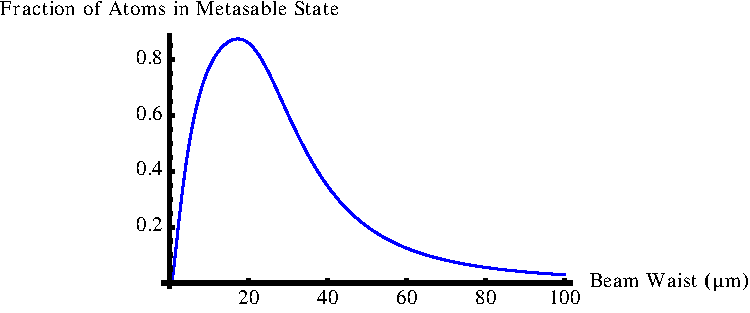
\includegraphics[width=6in]{MetaGraph1.pdf}
\caption{The fraction of atoms in the metastable state as a function of laser's beam waist. The fraction of atoms reaching the metastable state increases sharply as the beam waist increases until 20 microns. After 20 microns the number of atoms in the metastable state decreases because the atoms are ionizing.}
\label{MetaGraph1}
\end{figure}

Figure~\ref{AllGraph1} shows the fraction of atoms in each of the states which is helpful to see how the atoms move between states. The green line is the ground state which starts at one because the initial condition is all of the atoms in the ground state and continuously decreases as time passes. State 1 is the orange line; it quickly increases as atoms are excited through two-photon transition. The number of atoms in state 1 decrease as atoms decay either back to the ground state or to the metastable state. The number of atoms in the metastable state increases as atoms decay to it from the state 1. Atoms only leave the metastable state if they ionize. Only a small fraction of atoms are ionized, see the red line.

\begin{figure}[h!]
\centering
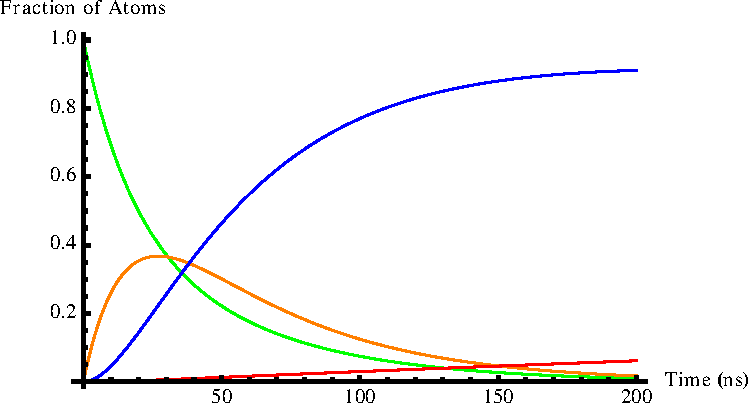
\includegraphics[width=6in]{AllGraph1.pdf}
\caption{The fraction of atoms in each state plotted against time. The green line is the ground state. The orange line is the excited $5P_{[3/2]_2}$ state. Blue is the metastable $5S_{[3/2]_2}$ and red is the fraction of atoms that have ionized.}
\label{AllGraph1}
\end{figure}

\subsection{Gaussian Beam Profile}

\subsection{Maxwell Velocity Distribution}

Adding the Maxwell velocity distribution presents new difficulties 
 
 

\section{Ti:Sapphire Laser}


\section{Laser Stabilization}




\begin{thebibliography}{0}



\end{thebibliography}


\end{document}
